\indent
In the last decades, we witnessed a growing demand for performing large-scale
computations, such as protein folding, fluid dynamics, weather and market prediction, or production process optimization.
The scale of such computations exceeds abilities of a single computer, hence they need to be performed on large sets of machines that cooperate over an interconnecting network, collectively called the \emph{computer cluster}.
Owning and maintaing large-scale computing infrastructure is often impractical and expensive, and parties look for alternative ways to perform computations.
In comparison, outsourcing computations provides a wide range of benefits.
First of all, it mitigates the costs of infrastructure management and maintenance.
This is crucial especially for computational tasks that arise occasionally, such as high-quality rendering, computer verification of products with long development time or analysis of human-harvested data.
Second, such approach dismisses the need to foresee the appropriate demand for resources.
If such demand increases unexpectedly, it can be immediately provided without physical extension of the infrastructure.
This led to a shift of computations to large-scale \emph{remote} facilites that contain computer clusters with their support infrastructure, the so-called \emph{data centers}.
Performing computations in these external data centers provides the impression of unlimited computational power on demand, and is called the \emph{cloud computing}.

The demand for outsourcing computations to the cloud created a whole market for such services.
Modern suppliers of processing power such as Microsoft Azure \cite{url-azure}, Amazon Elastic Cloud Computing EC2 \cite{url-amazon-ec2} or Google Compute Engine \cite{url-gce} provide convenient on-demand computational power while hiding most of details concerning resource management.
Processing capabilities are quickly and conveniently accessible to every interested party.

Computational tasks require multiple types of resources to complete: CPU time, memory, I/O operations and network bandwith.
Often the demand for these resources varies in time and is unpredictable.
For this reason, a data center that performs just one task at the time would waste resources.
In contrast, the co-existence of multiple tasks in the data center allows to compensate for the variable demand for resources by resource-aware scheduling.
Such techniques are especially useful in (but not limited to) computationally-intensive applications, where the response time is not the primary concern.

\textbf{The first part of this thesis assumes the perspective of a data center owner, whose main goal is an \emph{efficient management of resources}}.
For example, processing speed can be scaled down to save energy, memory can be shared or distributed, and cooperating processes can be migrated closer to each other in the network to save bandwidth.
In the first part of this thesis, we focus on the last aspect and we show how it leads to
\emph{efficient usage of an interconnecting network} in a data center.
Optimization of this resource is critical for performing efficient large-scale computations, as those involve multiple machines that cooperate over network.
To this end, we will make use of a~sophisticated control system, called \emph{virtualization}.


In the second part of this thesis, we shift our attention away from the optimization of data center network and focus on fundamental aspects of data transmission.
Data transmitted over a network is split into portions called packets, which are routed independently, and the task of relying a packet to its destination is called \emph{packet forwarding} and is performed by network devices called \emph{routers}.
Efficient packet forwarding is crucial in minimizing data transfer latency and maximizing the throughput.

Packet forwarding consists of series of relay operations between computer networks.
A single network is usually connected with multiple adjacent networks, and at each intermediate network a bordering router needs to determine the next network on the way of the packet.
To this end, such device directs packets based on the set of its forwarding rules (that represent the knowledge of the network about its surroundings).
The number of forwarding rules stored in the core Internet routers is almost as numerous as the total number of networks, which leads to enormous forwarding tables to manage.

In further sections, we elaborate more on consequences of large number of forwarding rules, and we investigate the increasingly common scenario, where the size of rules exceeds the available memory.
It is worth noting that networks can be either physical or virtual.
The concept of virtual networks described in Part~\ref{pt:virtual-networks} contributes immensely to partition of the Internet into subnetworks, and to growth of forwarding tables.

Nowadays, routers are often grouped in large facilities, called the \emph{Internet exchange points (IXP)}, that exchanges data on a large scale between large networks.
\textbf{The second part of this thesis assumes the perspective of IXP owner, whose objective is to \emph{maximize the efficiency of packet forwarding}.}


\section{Data Center Scenario: Machine Virtualization}
\sectionmark{Data Center Scenario}
\label{sec:intro-machine-virtualization}

Algorithmic techniques presented in the first part of this thesis rely upon logical isolation of a computation from the physical machine that performs the computation.
This gives a~possibility to manage the physical placement of a computation in a way that is transparent to the computation.
The rationality is that cooperating machines can be placed close to each other and close to the data they process.
A particular piece of technology that provides the flexibility in placement of computations is \emph{virtualization}.

Virtualization provides an abstraction layer for the underlying hardware of a computer system, called the \emph{virtual machine}.
Virtual machine mimics functionality of the physical hardware so closely and
directly that it can be used as an environment for a complete operating system.
Such operating system, running on a virtual machine is called the \emph{guest
operating system}. It operates in additon to the \emph{host operating
system}, which runs directly on the physical hardware. 

In a data center, the main purpose of virtualization is to provide the complete and non-restricted environment for the client that is isolated from the management software and other clients' tasks.
The guest operating system is restricted to the virtualized environment: it has the perspective of housing a whole computer system.


\subsection{Machine Migration}

Besides providing an abstraction layer, mature virtualization solutions suited for data center use such as Xen
\cite{url-xen}, KVM \cite{url-kvm}, Hyper-V \cite{url-hyperv}, VMware ESXi
\cite{url-vmware} provide several control features.
In particular, absolute control over the underlying virtual hardware allows to suspend and resume the execution of the guest operating system at will.
Such functionality provides building blocks for the feature of \emph{migration}, which transfers the complete virtual machine to a different physical machine.
This is possible without shutting down the guest operating system, and hence it provides a powerful resource-management tool that is transparent to clients.
Such mechanisms play an~important role in load balancing in the data center and allows for sophisticated optimizations such as \emph{reducing network distance between communicating virtual machines}.

Virtualization allows flexibility in renting infrastructure, and might offer savings in resource management.
However, an efficient use of resources requires sophisticated techniques to achieve its goal.
In this thesis, we focus on migration capabilities provided by modern virtualization techologies used for efficient usage of important resource in the data center --- the network bandwidth.
The problem central to the first part of this thesis is stated as follows:

\begin{center}
  \emph{How to assign virtual machines to physical machines to optimize network
  usage?}
\end{center}
We elaborate more in the subsequent subsection.

\subsection{Virtual Network Embedding}

Single virtual machine often provides insufficient resources for the client, as the resources of a~virtual machine are limited by resources available to its host.
Therefore, data centers provide its resources to clients as a sizeable set of virtual machines connected by a network.
Collectively, the virtual machines with their interconnecting network are called a \emph{virtual network}, where the cooperating virtual machines are refered to as \emph{nodes} of a virtual network.
To guarantee certain quality of service (\emph{QoS}) for multitude of co-existing virtual networks, up-front bandwidth reservations are required.
However, the generality of performed calculations results in unpredictibility of communication patterns and poses a challenge in optimization of bandwidth reservations.
In this thesis, we provide algorithms for efficient management of network reservations without any assumptions about communication patterns.

To measure the quality of resource management strategy, in Part~\ref{pt:virtual-networks} we state formal optimization problems; for now, we only briefly sketch it.
Physical components of a data center are often modelled in form of a~graph called a \emph{substrate network}, in which vertices correspond to physical machines, and edges correspond to an interconnecting network.
A communication cost between a pair of physical machines is proportional to edge-distance in substrate network (the number of \emph{hops} in the substrate network).
A communication pattern among virtual machines is also modelled as a graph, called a \emph{communication graph}.
In such settings, the communication among virtual machines running on certain physical machines can be viewed as a \emph{graph embedding} of communication graph into a substrate network~\cite{Goyal2008,gupta2001provisioning}.
The main objective is to find an embedding that locates closely the virtual machines that communicate often.

In this thesis, we study substrate networks in form of a tree, which closely models the popular Fat-Tree topology~\cite{fat-trees}.
In this tree topology, only leaves can host virtual machines, and the sole role of intermediate tree nodes is to transmit data between leaves, see Figure~\ref{fig:tree-topology}.


\begin{figure}[t]
\centering
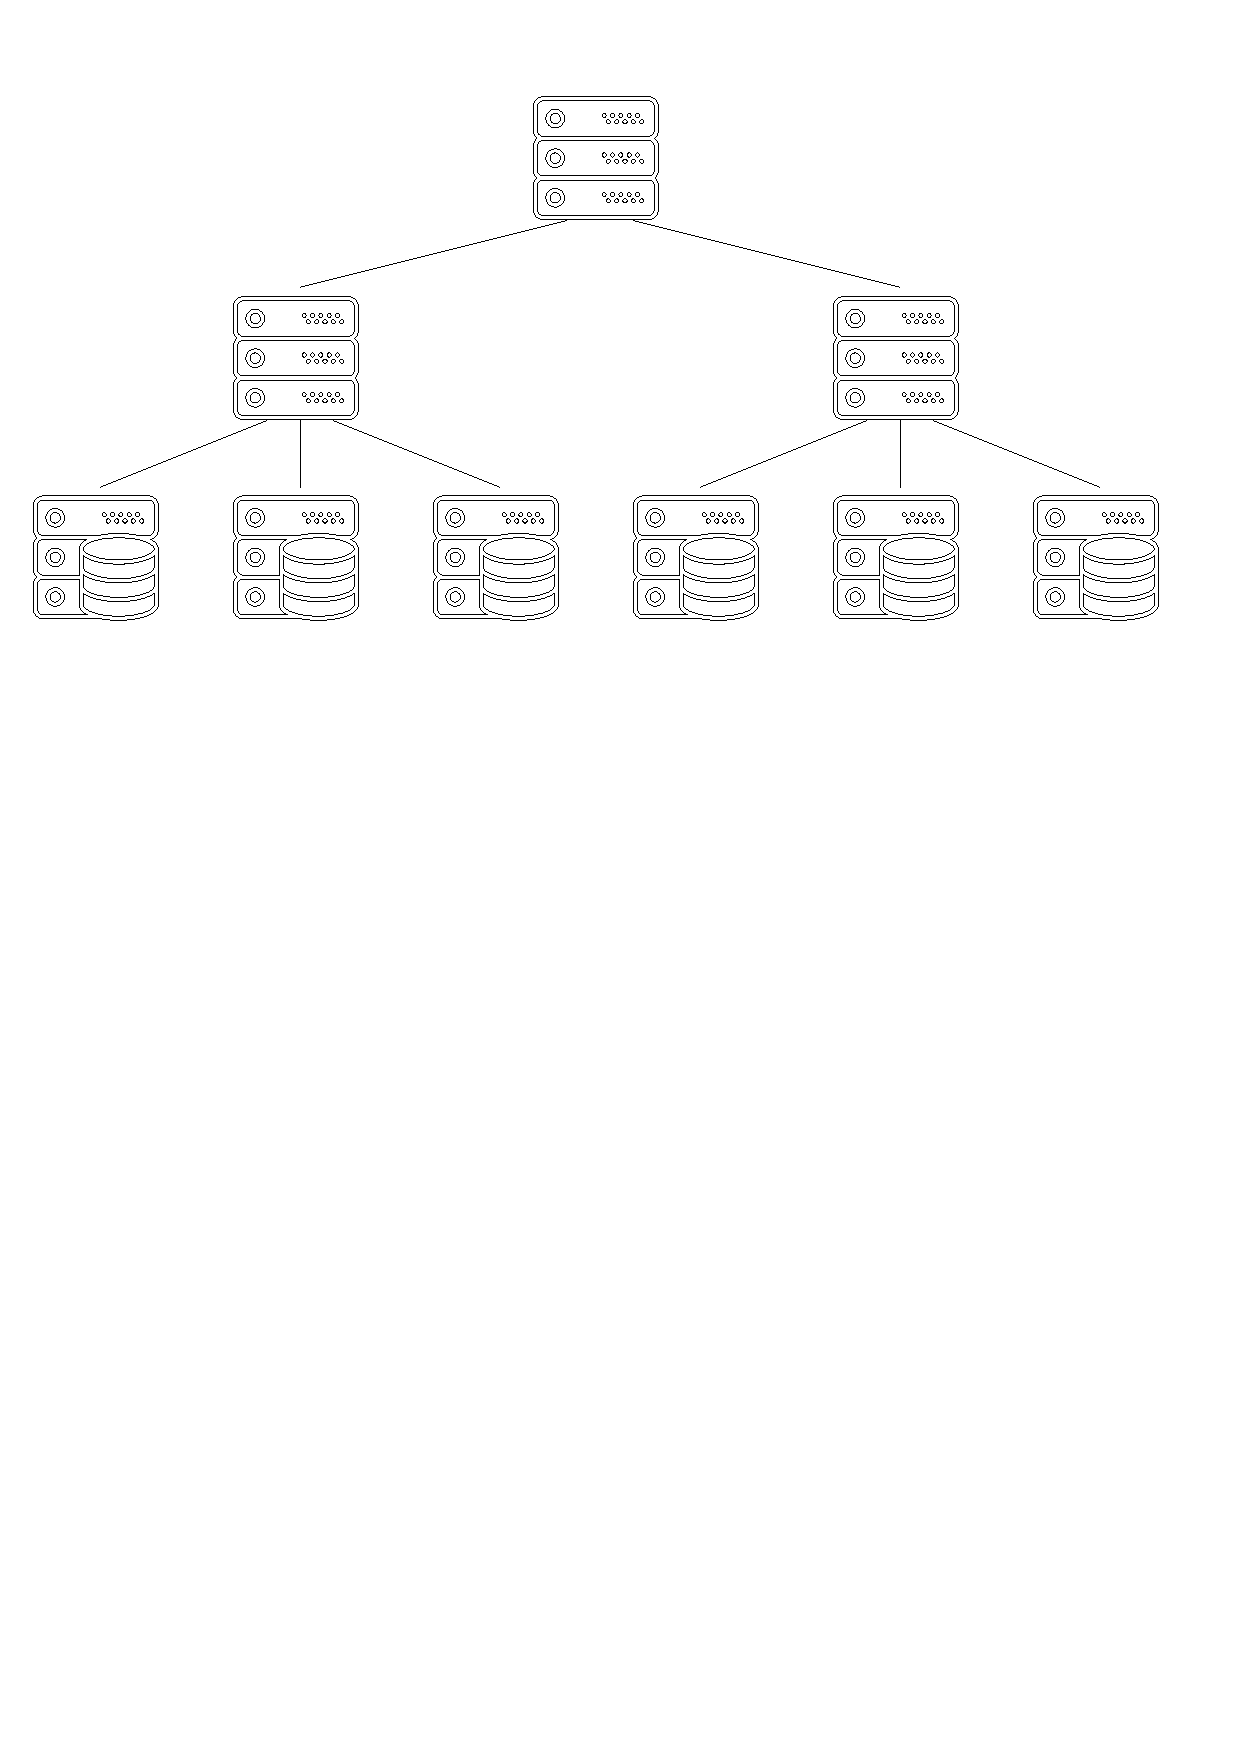
\includegraphics[width=0.79\columnwidth]{figs/tree-topology.pdf}
\caption{The model of typical data center with a tree-like network topology. We distinguish two types of tree nodes: the the intermediate nodes that transmit communication, and the computing machines, located at the leaves of a tree. Network links between nodes are depicted as solid lines.}\label{fig:tree-topology}
\vspace{-1em}
\end{figure}


\subsection{Our Contributions}

We consider two scenarios regarding virtual network embeddings:
\begin{enumerate}
  \item \emph{The static scenario}, where virtual machines are irrevocably assigned to their physical machines.
  \item \emph{The dynamic scenario}, where virtual machines can migrate between physical machines.
\end{enumerate}

We investigate the static scenario in Chapter~\ref{ch:static-mapping}, and the dynamic scenario in Chapter~\ref{ch:dynamic-mapping}.
Although the problems are related by their practical motivations, their combinatorial structure differs substantially.
In particular, the static scenario is not an offline version of the problem considered in the dynamic scenario.
In both scenarios, we assume that the communication pattern among virtual nodes is not known in advance.
In the static scenario we reserve a portion of bandwidth between every pair of virtual nodes to allow for any possible communication pattern.
On the other hand, in the dynamic scenario we react to changes in the communication pattern by migrating machines on the fly.
In addition, the problem considered in the static scenario is enriched by certain important properties of batch-processing applications that operate in distributed file systems.


\subsubsection{Static Mapping of Virtual Networks}
\label{sec:contributions-static-mapping}

In the static scenario studied in Chapter~\ref{ch:static-mapping}, to guarantee certain quality of service (\emph{QoS}), we need to acquire network reservations for all pairs of cooperating virtual machines.
The combinatorial problem that we consider in the static scenario is essentially a variant of the minimum-cost embedding of a clique (the communication graph) in a tree (the substrate network).
In addition, the scenario is designed to model certain aspects of MapReduce~\cite{mapreduce}, which is a predominant framework to perform large-scale, parallel data processing.
We consider the wide range of possible extensions that model certain aspects of Map-Reduce applications, most notably:

\begin{itemize}
\item \emph{Data chunk processing}. In Map-Reduce applications, virtual machines process large amounts of data chunks that are stored in a distributed file system. Each chunk of data must be assigned and transferred to a virtual machine. Data chunk transfer requires its own network reservations.

\item \emph{Data chunk replication}. Distributed file systems often store redundant copies of data chunks, called \emph{chunk replicas}. Only one copy of each data chunk replica must be processed, and we are free to choose the replica to be used based on its placement.

\item \emph{Bandwidth constraints}. Each link in substrate network has its capacity. For the embedding to be feasible, the total network reservations has to obey link capacities.
\end{itemize}


In particular, we decompose the general optimization problem into its fundamental aspects, such as
assignment of chunks, replica selection, and flexible virtual machine
placement, and answer questions such as:
\begin{enumerate}
\item Which chunks to assign to which virtual machine?

\item How to exploit redundancy and select good replicas?

\item How to efficiently embed virtual machines and their inter-connecting network?

\end{enumerate}

We draw a complete picture of the problem space: we show that
some problem variants (also those exhibiting multiple degrees of freedom in terms of
replica selection and embedding),
can be solved in polynomial time. For all other variants, we prove limitations in terms of
computational tractability, by proving their NP-completeness. Interestingly,
our hardness results also hold in \emph{uncapacitated}
networks of small-diameter networks (as they are
widely used today~\cite{fattree}).
We provide the full picture: for each considered variant we either provide a polynomial-time algorithm or we show that the problem is NP-hard.


\subsubsection{Dynamic Mapping of Virtual Networks}
\label{sec:contributions-dynamic-mapping}

In Chapter~\ref{ch:dynamic-mapping}, we study virtual network embeddings in the scenario where virtual machines can be migrated during runtime to another physical machine.
Possibility of migration provides efficient tools that allows to react to unpredictible communication patterns.
If some distant nodes communicate often, it is vital to reduce the distance to save network bandwidth.
The objective is to minimize the total network bandwidth used for communication and for migration.

We assume that the communication pattern is not known in advance.
We measure the quality of presented algorithmic solutions by competitive analysis~\cite{borodin-book}, which is well-suited for problems that are online by their nature.

In the dynamic scenario we assume that the physical substrate network takes a form of a~tree with height one.
Every physical machine (leaf) is connected directly to the root (that has no virtual machine hosting capabilities).
A single physical machine hosts a fixed number of virtual machines.

The model restricted to such networks becomes a variant of online graph clustering.
We are given a~set of~$n$ nodes with time-varying pairwise
communication patterns, which have to be partitioned into~$\ell$~clusters of
equal size~$k=n/\ell$. For example, in the context of~cloud computing, $n$ may represent virtual machines
or containers that are distributed across~$\ell$ physical servers, each having
$k$ cores: each server can host $k$ virtual machines.

We would like to
(dynamically) distribute the virtual machines across the servers such that
datacenter traffic and migration costs are minimized.
Intuitively, we would like to minimize inter-cluster
interactions by mapping frequently communicating nodes to the same cluster.
Since communication patterns change over time, partitions should be
readjusted dynamically, that is, the nodes should be \emph{repartitioned}, in
an online manner, by \emph{migrating} them between clusters. The objective is
to jointly minimize inter-cluster communication and repartitioning costs,
defined respectively as the number of communication requests ``served
remotely'' and the number of times nodes are migrated from one cluster to
another.


The possibility to perform a migration uncovers algorithmic challenges:
\begin{itemize}

\item \emph{Serve remotely or migrate?} For a brief communication
pattern, it may not be worthwhile to collocate the nodes: the migration might
be too large in comparison to communication costs.

\item \emph{Where to migrate, and what?}
If an algorithm decides to collocate nodes $x$ and~$y$, the question becomes
how. Should $x$ be migrated to the cluster holding $y$, $y$ to the one holding
$x$, or should both nodes be migrated to a new cluster?

\item \emph{Which nodes to evict?}
There may not exist sufficient space in the desired destination cluster. In
this case, the~algorithm needs to decide which nodes to ``evict'' (migrate to
other clusters), to free up space.

\end{itemize}

In the considered model, every physical machine fully utilizes its processing capabilities --- it hosts maximum possible amount of virtual machines, i.e. $k=n/\ell$.
Hence, the migration is not possible without the further reconfigurations: to respect physical machine capacity, we need to decide which virtual machines to swap.
For this setting, we show deterministic lower-bound of $k$, where $k$ is the physical machines hosting capacity.
We present constant-competitive algorithm for the scenario restricted to physical machines that host two virtual machines ($k = 2$).

In this chapter, we also consider the resource-augmentation scenario, where we relax this assumption: the total hosting capacity of physical machines exceeds the total number of virtual machines, i.e. $k > n/\ell$.
The main contribution of this part is an efficient algorithm for the scenario with small resource augmentation.

%This fundamental online optimization problem has many applications. For
%example, in the context of~cloud computing, $n$ may represent virtual machines
%or containers that are distributed across~$\ell$ physical servers, each having
%$k$ cores: each server can host $k$ virtual machines. We would like to
%(dynamically) distribute the virtual machines across the servers such that
%datacenter traffic and migration costs are minimized.


\subsection{Related Work}


Recently, there has been much interest in programming models and distributed
system architectures for the processing and analysis of big data (e.g.~\cite{nodb,mapreduce,shark}).
Such applications
generate large amounts of network traffic~\cite{orchestra,talk-about,amazonbw},
and over the last years, several systems have been proposed which provide
a provable network performance, also in shared cloud environments, by supporting
relative~\cite{faircloud,elasticswitch,seawall}
or, as in the case of this thesis, \emph{absolute}~\cite{oktopus,secondnet,drl,gatekeeper,proteus} bandwidth reservations
between the virtual machines.

In Chapter~\ref{ch:static-mapping} we study static virtual network embeddings.
Our model is enriched by motivations that follow from batch-processing applications~\cite{mapreduce}.
The most popular virtual network abstraction for such applications today is the \emph{virtual cluster}~\cite{oktopus}, later studied by many others~\cite{talk-about,infocom16,ccr15emb,proteus}.
From a theoretical perspective, the virtual network embedding problem can be seen as a generalization
of classic VPN graph embedding problems~\cite{Goyal2008,gupta2001provisioning}, which requires finding a graph embedding with fixed endpoints.
In virtual network embedding problems studied in this thesis, the embedding endpoints are the subject to optimization.
In this respect, the virtual network embedding problem can also be seen as related to
classic Minimum Linear Arrangement problem~\cite{mla,mla-survey} which asks for the
embedding of guest graphs on a simple \emph{line topology} (rather than tree-like topologies as
studied in this thesis).


The online problem considered in Chapter~\ref{ch:dynamic-mapping} was not previously studied.
However, the static offline version of the problem, i.e., a problem variant where
migration is not allowed, where all requests are known in advance, and where
the goal is to find best node assignment to $\ell$~clusters, is known as the
\emph{$\ell$-balanced graph partitioning problem}. The problem is 
NP-complete, and cannot even be approximated within any finite factor unless P
= NP~\cite{AndRae06}.  The static
variant where $\ell = 2$ corresponds to the minimum bisection problem, which
is already NP-hard~\cite{GaJoSt76}.
Its approximation was studied in a long
line of work~\cite{SarVaz95,ArKaKa99,FeKrNi00,FeiKra02,KraFei06,Raec08} and
the currently best approximation ratio of $O(\log n)$ was given by
R{\"{a}}cke~\cite{Raec08}.
The inaproximability of the static variant for general values of $\ell$
motivated research on the bicriteria variant, which can be seen as the offline
counterpart of our cluster-size augmentation approach. Here, the~goal
is~to~develop $(\ell,\delta)$-balanced graph partitioning, where the graph has
to be partitioned into $\ell$ components of~size less than $\delta \cdot (n /
\ell)$ and the cost of the cut is compared to the optimal (non-augmented)
solution where all components are of size~$n / \ell$. The variant where
$\delta \geq 2$ was considered in
\cite{LeMaTr90,SimTen97,EvNaRS00,EvNaRS99,KrNaSc09}. So far, the best result is
an $O(\!\sqrt{\log n \cdot \log \ell})$-approximation by Krauthgamer et
al.~\cite{KrNaSc09}, which builds on ideas from the $O(\!\sqrt{\log
n})$-approximation algorithm for balanced cuts by Arora et al.~\cite{ArRaVa09}.

\begin{large}
  PONIZEJ WERSJA Z PRACY DLA POROWNANIA
\end{large}

Our model is related to online
paging~\cite{SleTar85,FKLMSY91,McGSle91,AcChNo00}, sometimes also referred to
as online caching, where requests for data items (nodes) arrive over time and
need to be served from a cache of finite capacity, and where the number of
cache misses must be minimized. Classic problem variants usually boil down to
finding a smart eviction strategy, such as Least Recently Used (LRU). In our
setting, requests can be served remotely (i.e., without fetching the
corresponding nodes to a single cluster). In this light, our model is more
reminiscent of caching models \emph{with
bypassing}~\cite{EpImLN11,EpImLN15,Irani02}. Nonetheless, we show that BRP is
capable of emulating online paging.

The dynamic embedding problem studied in this thesis is an example of a non-uniform problem~\cite{KaMaMO94}: the
cost of changing the state is higher than the cost of serving a single
request. This requires finding a~good trade-off between serving requests
remotely (at a low but repeated communication cost) or migrating nodes into a
single cluster (entailing a potentially high one-time cost). Many
online problems exhibit this so called \emph{rent-or-buy} property, e.g., ski
rental problem~\cite{KaMaMO94,LoPaRa08}, relaxed metrical task
systems~\cite{BaChIn01}, file migration~\cite{BaChIn01,BiByMu17}, distributed
data management~\cite{BaFiRa95,AwBaFi93,AwBaFi98}, or rent-or-buy network
design~\cite{AwAzBa04,Umboh15,FeWiLe16}.

There are two major differences between the dynamic embedding problem and the problems listed above.
First, these problems typically maintain some configuration of servers or
bought infrastructure and upon a new request (whose cost typically depends on
the distance to the infrastructure), decide about its reconfiguration (e.g.,
server movement or purchasing additional links). In contrast, in our model,
\emph{both} end-points of a communication request are subject to optimization.
Second, in the dynamic embedding problem a request reveals only very limited information
about the optimal configuration to serve it: There exist relatively long
sequences of requests that can be served with zero cost from a fixed
configuration. Not only can the set of such configurations be very large, but
such configurations may also differ significantly from each other.



\section{Internet Exchange Point Scenario: Router Memory Optimization}
\sectionmark{Internet Exchange Point Scenario}
\label{sec:intro-packet-forwarding}

In the second part of this thesis, we consider the fundamental problem of \emph{packet forwarding}.
We focus on a single router, that physically connects different networks and is responsible for passing packets between them.
Upon receiving a data packet, the router forwards it to a specific output port leading to a neighbouring network.
To choose the appropriate port, the router stores of a \emph{forwarding table}, which consists of rules describing how to map the packet destination addresses to appropriate ports.

The router maintains the forwarding table in its memory.
Only a small restricted set of operations is performed on such memory: lookups and updates.
Nowadays, routers perform milions of lookup operations and thousands updates~\cite{bgp-updates}, and the utilizing specialized hardware is crucial for the efficiency of packet forwarding.
Hence, instead of relying on the general-purpose memory such as RAM (where lookup operation is costly), the specialized memory units such as TCAM~\cite{tcam-memory} are utilized.
The TCAM memory is an associative memory storage with a variation of pattern-matching lookup that closely matches the way the forwarding rules are used.

With the growth of the Internet, the number of connected networks increases with rapid progression, which often induces new forwarding rules to store.
In effect, the size of forwarding table exceeds the amount of available TCAM memory in a typical router (the phenomenon called the TCAM exhaustion~\cite{tcam-exhaust}).
Sophisticated electronics circuits such as TCAM are very expensive in comparison to RAM and
power-hungry~\cite{tcam-expensive}.
Typical operations performed on TCAM memory examine the whole contents stored in memory, which requires closely connected physical structure among memory cells --- as the result, it is expensive to expand available memory.

Internet exchange points are located in the core of the Internet, and their routers forward packets among large number of networks.
Hence, their forwarding tables usually contain forwarding entries for all of them.
In Figure~\ref{fig:bgp-entries}, we see the growth of the number of entries in the global forwarding table \cite{url-bgp-entries}.
Size of forwarding tables of the routers in the core of the Internet are approaching such size.
Those routers have to store an~enormous number of forwarding rules: the
number of rules has doubled in the last six years~\cite{bgp-routeviews} and
the superlinear growth is likely to be sustained~\cite{steve-myth}.


Limited size of memory and expanding size of the content to store brings new challenges in memory management of the routers.
In the second part of this thesis, we investigate the following problem, using the tools provided by contemporary routers:
\begin{center}
  \emph{How to efficiently manage the memory of forwarding devices?}
\end{center}


\begin{figure}[t]
\centering
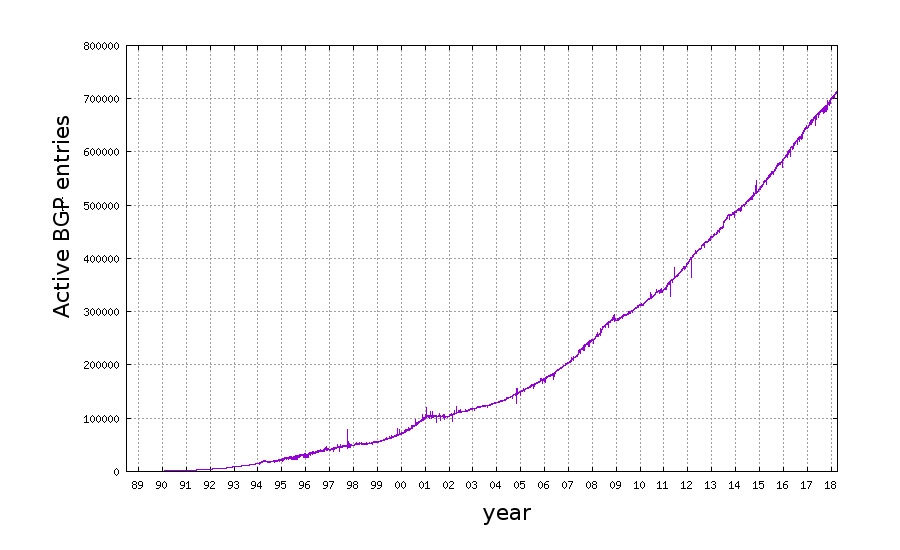
\includegraphics[width=0.59\columnwidth]{figs/bgp-entries.png}
\caption{The number of entries in the global forwarding table. The global forwarding table is built upon the informations exchanged via Border Gateway Protocol. The graph presents the growth of the global forwarding table from 1988 to 2018.}\label{fig:bgp-entries}
\vspace{-1em}
\end{figure}

\subsection{Caching of Forwarding Rules}

A~solution, which could delay
the need for expensive or impossible memory upgrades in routers, is to store
only a subset of rules in the actual router and store all rules on a~secondary
device (for example a commodity server with a large but slow
memory)~\cite{cacheflow,route-caching-flat,prefix-caching,fib-caching-non-overlapping,fibium-zipf}.
This solution is particularly attractive with the advent of Soft\-ware-Defined
Network (SDN) technology, which allows to manage the expensive memory using a
software controller~\cite{cacheflow,fibium-zipf}. In particular, our
theoretical model can describe real-world architectures
like~\cite{cacheflow,fibium-zipf},
that is, our model formalizes the underlying operational
problems of such architectures. Our 
algorithm, when applied in the context of such architectures, can 
hence be used to prolong the lifetime of IP routers.


In the second part of this thesis, we consider the problem of memory management in routers.
Modern routers consist of two logical components. Those two components use disjoint memory (often of distinct type) and disjoint processing units:
\begin{enumerate}
  \item The forwarding plane, which  contains forwarding table described in the previous section, and performs the actual packet transmission according to the forwarding table.
  \item The control plane, which is responsible for reflecting the network topology in the forwarding table.
\end{enumerate}

The forwarding component has finite memory, and in multiple scenarios the size of forwarding table exceeds the size of available memory.
One of the solutions is to store only a part of a~forwarding table on the forwarding device, that acts as a cache for the complete forwarding table that is stored in the control plane, see Figure~\ref{fig:router}.
However, this might result in the situation, where the forwarding device do not posess sufficient information to proceed (\emph{a cache miss}).

Even upon the cache miss, the packet still needs to reach its destination.
The common way to handle the situation is to redirect the packet to the control plane component, which posseses the complete forwarding table.
However, the packet cannot be forwarded by the control plane, hence it is supplemented with forwarding informations and sent back to the forwarding plane.
The forwarding device overrides the usual procedure of forwarding table lookup, and instead it uses the supplemented information to forward the packet.


\begin{figure}[t]
\centering
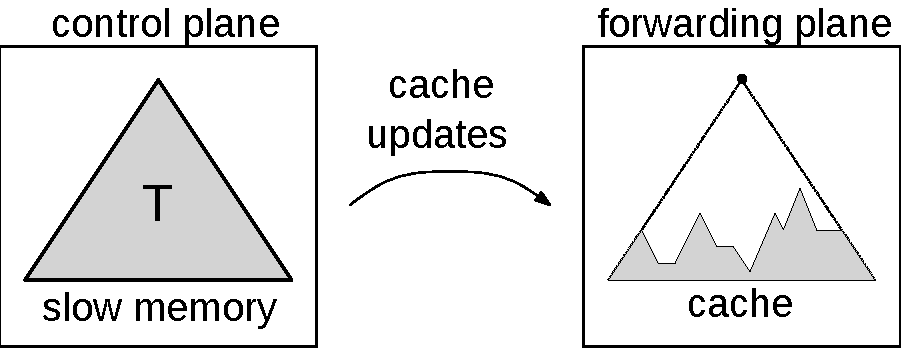
\includegraphics[width=0.59\columnwidth]{figs/router5.pdf}
\caption{We propose a caching scenario, where the limited memory of a router stores a portion of the forwarding table. The complete forwarding table is stored at the controller.}\label{fig:router}
\vspace{-1em}
\end{figure}




Upon the forwarding table cache miss, the control plane may decide to update the cached portion of the forwarding table that resides in the forwarding component.
Standard caching-related problems arise, such as: which entry to evict to provide space to store the new entry.
Immediate update might seem a rational strategy, but in scenarios with highly dynamic networks that rearrange often, it might be beneficial to delay the update.
Premature update might result in the situation, where more time is spent alternating the cache configuration than processing packets (this is similar to \emph{thrashing} in virtual memory systems).

In the traditional caching problem, the cache elements are independent: it is always feasible to pull in or out the elements of the cache regardless of cache configuration.

Note that the technical feasibility of this solution heavily depends on the
rule dependencies. In the most ubiquitous scenario, the rules are prefixes of
IP addresses (they are bit strings). Whenever a packet arrives, the router
follows a longest matching prefix (LMP) scheme: it searches for the rule that
is a~prefix of the destination IP of the packet and among matching rules it
chooses the longest one. In other words, if the prefixes corresponding to
rules are stored in the tree\footnote{We do not have to assume that they are
actually stored in a real tree; this tree is implicit in the LMP scheme.},
then the tree is traversed from the root downwards, and the last found rule is
used. This explains why we require the cached nodes to form a subforest:
leaving a less specific rule on the router while evicting a more specific one
(i.e., keeping a~tree node in cache while evicting its descendant) will result
in a~situation where packets will be forwarded according to the less specific
rule, and hence potentially exit through the wrong port. The LMP scheme also
ensures that the described approach is implementable: one could simply add
an~artificial rule at the tree root in the router (matching an empty prefix).
This ensures that when no actual matching rule is found in the router (in the
cache), the packet will be forwarded according to this artificial rule to the
controller that stores all the rules and can handle all packets appropriately.

Additionally, a rule may need to be updated. For example, due to a~change
communicated by a dynamic routing protocol (e.g., BGP) the action defined by
a~rule has to be modified. In either case, we have to update the rules at the
controller: we assume that this cost is zero. (This cost is unavoidable for
any algorithm, so such an assumption makes our problem only more difficult.)
Furthermore, if the rule is also stored at the router, then we have to pay a~fixed
cost of $\alpha$ for updating the router (see the remark for the cost of
fetches and evictions). Such penalties can be easily simulated in our model:
we issue a~sequence of $\alpha$ negative requests to the updated node.  It is
straightforward to show that the costs in these two models can differ by a
factor of at most $2$. For a~formal argument, see
\lref[Appendix]{sec:bisimulation}.




In contemporary networks, the control plane component can be physically separated from the forwarding plane, and to perform remote management over the network it uses protocols such as OpenFlow~\cite{openflow}.
In such scenario, excessive cache updates cause not only delay in packet processing, but also cause congestion in the network between the forwarding component and the control component.

Caching scenarios are best expressed and analysed in online settings.
Similarly to Chapter~\ref{ch:dynamic-mapping}, we use the competitive analysis to determine the performance of our strategy~\cite{borodin-book}.
In this thesis, we consider the variant of caching with dependencies among cached elements motivated by the structure of forwarding table.


\subsection{Our Contributions}

%We initiate the study of a natural new caching with bypassing problem which
%allows to account for tree-dependencies among items. The problem finds
%immediate applications, e.g., in IP routing and software-defined networking
%(see \lref[Section]{sec:motivation}).
%
%In particular, we consider the online tree caching problem within the resource
%augmentation paradigm: we assume that cache sizes of the online algorithm
%($\kALG$)  and the optimal offline algorithm ($\kOPT$) may differ. We assume
%$\kALG \geq \kOPT$ and let $R = \kALG/(\kALG-\kOPT+1)$.

In \lref[Section]{sec:algo}, we present an elegant deterministic online
algorithm~\ALG for this problem. While our algorithm is simple, its analysis
presented in \lref[Section]{sec:analysis} requires several non-trivial
insights into the problem. In particular, we rigorously prove that \ALG is
$O(h(T) \cdot R)$-competitive, where $h(T)$ is the height of tree~$T$. That
is, we show that there exists a constant~$\beta$, such that $\ALG(I) \leq
O(h(T) \cdot R) \cdot \OPT(I) + \beta$ for any input $I$. Note that this
result is optimal up to the factor~$O(h(T))$: in
\lref[Appendix]{sec:lower-bound-on-the-problem}, we show that the lower
bound~$R$ for the paging problem~\cite{competitive-analysis} implies an
$\Omega(R)$ lower bound for our problem for any $\alpha \geq 1$. Finally, in
\lref[Section]{sec:implementing_counters}, we show that \ALG can be
implemented efficiently.


\subsection{Related Work}

Our formal model is a novel variant of competitive paging, a~classic online
problem. In the framework of the competitive analysis, the paging problem was
first analyzed  by Sleator and Tarjan~\cite{competitive-analysis} $k$-competitive algorithms (where $k$ is the cache size) and a matching lower-bound.
The simple paging problem was later generalized to allow different fetching
costs (weighted paging)~\cite{double-coverage,young-paging-greedy-dual} and
additionally different item sizes (file caching)~\cite{young-paging-landlord},
with the same competitive ratio.
%Asymptotically same results can be achieved
%when bypassing is allowed (see \cite{caching-rejection-penalties,paging-irani}
%and references therein).
To the best of our knowledge, the variant of caching, where fetching items to
the cache is not allowed unless some other items are cached (e.g., because of 
tree dependencies) was 
not considered previously in the framework of competitive analysis.

Other approaches for minimizing the number of stored rules were mostly based
on \emph{rules compression (aggregation)}, where the set of rules was replaced
by another equivalent and smaller set. Optimal aggregation of a fixed routing
table can be achieved by dynamic
programming~\cite{ortc,fib-compression-two-dimensional}, but the main
challenge lies in balancing the achieved compression and the amount of changes
to the routing table in the presence of \emph{updates} to this table. While
many practical heuristics have been devised by the networking community for
this problem~\cite{mms,fib-compression-fifa,fib-compression-globecom10,fib-compression-infocom13,fib-sigcomm,fib-compression-smalta,fib-compression-infocom10},
worst-case analyses were presented only for some restricted
scenarios~\cite{fib-icdcs,fib-sirocco}. Combining rules compression and rules
caching is so far an unexplored area.


So far, the papers on IP rule caching avoided dependencies either assuming
that rules do not overlap (a~tree has a single level)~\cite{route-caching-flat} 
or by preprocessing the tree, so that the rules become
non-overlapping~\cite{prefix-caching,fib-caching-non-overlapping}.
Unfortunately, this could lead to a large inflation of the routing table. A
notable exception is a recent solution called CacheFlow~\cite{cacheflow}. The
CacheFlow model supports dependencies even in the form of directed acyclic
graphs. However, CacheFlow was evaluated only experimentally, and no
worst-case guarantees were given on the overall cost of caching. Our work
provides theoretical foundations for respecting tree dependencies.



\section{Bibliographic notes and acknowledgements}

The results of this thesis were published by the author of this thesis in various conferences and journals.
Parts of Chapter~\ref{ch:static-mapping} appeared previously in the proceedings of 23rd IEEE International Conference on Network Protocols (ICNP 2015)~\cite{my-icnp},
and in Theoretical Computer Science, vol.~697~\cite{my-tcs}.
Some of the results from Chapter~\ref{ch:static-mapping} appeared in the PhD thesis of my co-author Carlo Fuerst.
Parts of Chapter~\ref{ch:dynamic-mapping} appeared previously in the proceedings of 30th International Symposium on Distributed Computing (DISC 2016)~\cite{my-disc}, and parts of Chapter~\ref{ch:packet-forwarding} --- in the proceedings of 29th ACM Symposium on Parallelism in Algorithmics and Architectures (ACM~SPAA~2017)~\cite{my-spaa}.
Preliminary results from Chapter~\ref{ch:packet-forwarding} appeared in the master thesis of my co-author Aleksandra Spyra.

For some figures in this thesis, icons by Smashicons from www.flaticons.com were used.